\textbf{See the instruction for questions \inteval{\value{question}+1} to \inteval{\value{question}+2}.}

\begin{figure}[H]
\centering
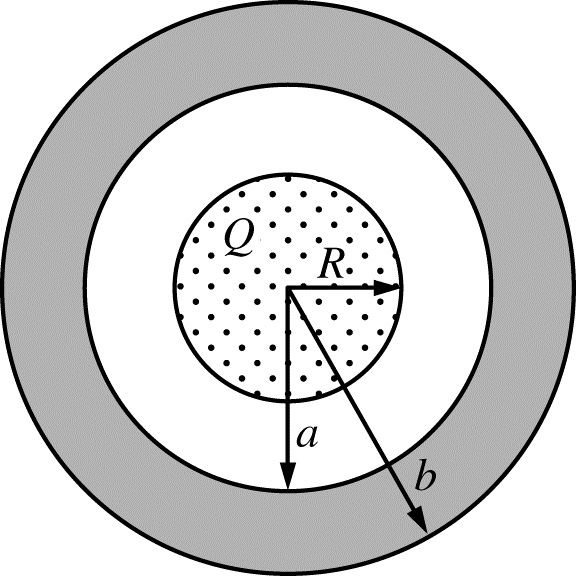
\includegraphics[scale=0.25]{images/img-006-020.png}
\end{figure}

An insulated nonconducting sphere of radius $R$ has a charge $Q$ uniformly distributed throughout its volume. It is surrounded by a concentric spherical conducting shell of inner radius $a$ and outer radius $b$, as shown in the figure above. There is no net charge on the conducting shell. Let $E$ be the electric field magnitude at a distance $r$ from the center of the spheres.

% Multiple Choice Question 8
\begin{questions}\setcounter{question}{7}\question
Which of the following represents a correct application of Gauss's law for $r>b$ ?

\begin{choices}
\choice $0=E(4 \pi) r^{2}$
\choice $\dfrac{Q}{\epsilon_{0}}=E(4 \pi) r^{2}$
\choice $\dfrac{Q}{\epsilon_{0}}=E(4 \pi) R^{2}$
\choice $\dfrac{Q r^{3}}{\epsilon_{0} R^{3}}=E(4 \pi) r^{2}$
\choice $\dfrac{Q a^{3}}{\epsilon_{0} R^{3}}=E(4 \pi) r^{2}$
\end{choices}\end{questions}

% Multiple Choice Question 9
\begin{questions}\setcounter{question}{8}\question
Which of the following represents a correct application of Gauss's law for $r<R$ ?

\begin{choices}
\choice $0=E(4 \pi) r^{2}$
\choice $\dfrac{Q}{\epsilon_{0}}=E(4 \pi) r^{2}$
\choice $\dfrac{Q}{\epsilon_{0}}=E(4 \pi) R^{2}$
\choice $\dfrac{Q r^{3}}{\epsilon_{0} R^{3}}=E(4 \pi) r^{2}$
\choice $\dfrac{Q a^{3}}{\epsilon_{0} R^{3}}=E(4 \pi) r^{2}$
\end{choices}\end{questions}

